%README file for moduleDocumentationTemplate TeX template.
%This template should be used to document all Basilisk modules.
%Updated 20170711 - S. Carnahan
%
%-Copy the contents of this folder to your own _Documentation folder
%
%-Rename the Basilisk-moduleDocumentationTemplate.tex appropriately
%
%-All edits should be made in one of:
%—header.tex
%— modelAssumptionsLimitations.tex
%— modelDescription.tex
%— modelFunctions.tex
%— revisionTable.tex
%— testDescription.tex
%— testParameters.tex
%— testResults.tex
%— user_guide.tex
%
%-Some rules about referencing within the document:
%1. If writing the suer guide, assume the module description is present
%2. If writing the validation section, assume the module features section is present
%3. Make no other assumptions about any sections being present. This allow for sections of the document to be used elsewhere without breaking.

%In order to import some of these sections into a document in a different directory:
%\usepackage{import}
%Then, the sections are called with \subimport{relative path}{file} in order to \input{file} using the right relative path.
%\import{full path}{file} can also be used if absolute paths are preferred over relative paths.

%%%%%%%%%%%%%%%%%%%%%%%%%%%%%%%%%%%%%%%%%%%%%%%%%%%%%%%%%%%%%%%%%%%%%%%%%%%%%
%%%%%%%%%%%%%%%%%%%%%%%%%%%%%%%%%%%%%%%%%%%%%%%%%%%%%%%%%%%%%%%%%%%%%%%%%%%%%
%%%%%%%%%%%%%%%%%%%%%%%%%%%%%%%%%%%%%%%%%%%%%%%%%%%%%%%%%%%%%%%%%%%%%%%%%%%%%


\documentclass[]{BasiliskReportMemo}

\usepackage{cite}
\usepackage{AVS}
\usepackage{float} %use [H] to keep tables where you put them
\usepackage{array} %easy control of text in tables
\usepackage{import} %allows for importing from multiple sub-directories
\bibliographystyle{plain}


\newcommand{\submiterInstitute}{Autonomous Vehicle Simulation (AVS) Laboratory,\\ University of Colorado}


\newcommand{\ModuleName}{SphericalHarmonics}
\newcommand{\subject}{Spherical Harmonics C++ model}
\newcommand{\status}{Tested}
\newcommand{\preparer}{S. Carnahan}
\newcommand{\summary}{The gravity effector module is responsible for calculating the effects of gravity from a body on a spacecraft. A spherical harmonics model and implementation is developed and described. A unit test has been written and run which tests basic input/output, single-body gravitational acceleration, and multi-body gravitational acceleration.}

\begin{document}

\makeCover

%
%	enter the revision documentation here
%	to add more lines, copy the table entry and the \hline, and paste after the current entry.
%
\pagestyle{empty}
{\renewcommand{\arraystretch}{2}
	\noindent
	\begin{longtable}{|p{0.5in}|p{3.5in}|p{1.07in}|p{0.9in}|}
		\hline
		{\bfseries Rev} & {\bfseries Change Description} & {\bfseries By}& {\bfseries Date} \\
		\hline
		1.0 & First version - Mathematical formulation and implementation & M. Diaz Ramos & 20170101\\
		\hline
		1.1 & Added test documentation & S. Carnahan &20170713\\
		\hline
		
	\end{longtable}
}

\newpage
\setcounter{page}{1}
\pagestyle{fancy}

\tableofcontents %Autogenerate the table of contents
~\\ \hrule ~\\ %Makes the line under table of contents
	
\section{Model Description}

This utility produces white noise. It can have a bias added to it to make a non-zero mean. It also generates "random walk" by treating the noise as additive. Walk bounds can be provided that push the random walk away from the boundary. Setting the bounds to zero or less disables the random walk, this is the default.
 %This section includes mathematical models, code description, etc.

\section{Model Functions}
The mathematical description of gravity effects are implemented in gravityEffector.cpp. This code performs the following primary functions
\begin{itemize}
	\item \textbf{Cannonball Method}: The code calculates the force on a spacecraft due to solar radiation pressure.
	\item \textbf{Look-up Method}: The code calculates both the force and torque on a spacecraft due to solar radiation pressure. It uses user-provided tabulated data to do so.
	\item \textbf{Solar Eclipse}: The code takes solar eclipses into account via a "shadow factor". This shadow factor is output from the Basilisk solar eclipse module and can include the effects of multiple planets. It is applied to the force/torque outputs.
	\item \textbf{Interface: Spacecraft States}: The code receives spacecraft state information via the DynParamManager.
	\item \textbf{Interface: Forces and Torques}: The code sends spacecraft force and torque contributions via computeForceTorque() which is called by the spacecraft.	If using the cannonball method, the returned torque values are zero.
	\item \textbf{Interface: Sun Ephemeris}: The code receives Sun states (ephemeris information) via the Basilisk messaging system.
	\item \textbf{Interface: Solar Eclipse}: The code receives solar eclipse (shadow factor) information via the Basilisk messaging system.
	
\end{itemize}



\section{Model Assumptions and Limitations}
The two methods of calculation used in this code have their own sets of assumptions and limitations. There are some assumptions which are common to both methods.
\begin{itemize}
	\item \textbf{Cannonball Model}: This default solar radiation pressure model assumes that the radiation pressure will act normal to some equivalent surface area, $A_{\odot}$. While this could be a good assumption, $A_{\odot}$ would have to be time-varying with spacecraft attitude and incorporate spacecraft self-shadowing. In general, the code does not do this. This limits the cannonball method to being most accurate in relatively mundane simulations (no rapid rotations or varying self-shadowing). Additionally, this method does not calculate torques on the spacecraft, so it is limited to cases where high precision is not needed with regards to spacecraft attitude.
	\item \textbf{Look-up Method}: This method utilizes tabulated data. Therefore, there will be error associated with whatever method was used to generate and record the data, but those errors are outside of Basilisk. Furthermore, the algorithm selects the data which \textit{most closely} matches the current position of the spacecraft relative to the sun and does not interpolate between data points.  This method also is limited to users who have external models or real data to use to describe their spacecraft.
	\item \textbf{Radiation}: The radiation model is hard-coded to assume that the radiation comes from the Sun. It is not possible to model radiation pressure from other sources with this code. This applies to both the cannonball and look-up methods. The model has no time-varying radiation effects (solar storms, etc.). A more in-depth radiation model would be need if high-accuracy radiation pressure effect calculations are needed.
	\item \textbf{Eclipse}: The shadow factor applies a simple scaling factor to the output forces and torques. This assumes that all portions of the spacecraft are affected equally by the eclipse. This should, in most circumstances, be highly accurate. For exceptionally large $A_{\odot}$ spacecraft which also need highly accurate state calculations, this assumption could fail.
	\item \textbf{Tabulated Data Import} Currently, Basilisk includes a utility script to import data from XML files for use in radiation pressure calculations. While some users could learn to load data in other formats, this is currently a limitation to most users who have data in other forms.
\end{itemize} %This includes a concise list of what the module does.

% !TEX root = ./Basilisk-MODULENAME-yyyymmdd.tex


\section{Model Assumptions and Limitations}
This section should describe the assumptions used in formulating the mathematical model and how those assumptions limit the usefulness of the module. %This explains the assumptions made to reach the final mathematical implementation of the model and how those assumptions limit the model's usefulness.

\section{Test Description and Success Criteria}
This test is located in \tt SimCode/dynamics/HingedRigidBodies/UnitTest/\newline
test\_hingedRigidBodyStateEffector.py. In this integrated test there are two hinged rigid bodies connected to the spacecraft hub. Energy and momentum are the primary methods for validation. Depending on the scenario, however, there are different success criteria. These are outlined in the following list:
\begin{itemize}
	\item Gravity and no damping scenario:
	\subitem Conservation of orbital angular momentum
	\subitem Conservation of orbital energy
	\subitem Conservation of rotational angular momentum
	\subitem Conservation of rotational energy
	\subitem Achieving the expected final attitude
	\item No gravity and no damping scenario:
\subitem Conservation of orbital angular momentum
\subitem Conservation of orbital energy
\subitem Conservation of rotational angular momentum
\subitem Conservation of rotational energy
\subitem Achieving the expected final attitude (same final attitude as the Gravity with no damping scenario)
\subitem Achieving the expected final position
\subitem Conservation of velocity of center of mass
	\item No gravity with damping scenario:
\subitem Conservation of orbital angular momentum
\subitem Conservation of orbital energy
\subitem Conservation of rotational angular momentum
\subitem Conservation of velocity of center of mass

\end{itemize}
 %This explains the unit test for the model. I.e. what features are tested and how. It may also include test tolerances, etc.

\section{Test Parameters}

This section summarizes the error tolerances for each test. Error tolerances are determined based on whether the test results comparison should be exact or approximate due to integration or other reasons. Error tolerances for each test are summarized in table \ref{tab:errortol}. 

\begin{table}[htbp]
	\caption{Error tolerance for each test.}
	\label{tab:errortol}
	\centering \fontsize{10}{10}\selectfont
	\begin{tabular}{ c | c } % Column formatting, 
		\hline
		\textbf{Test}   	      	               & \textbf{Tolerated Error} 						           \\ \hline
		``Cannonball"                           &\input{AutoTex/cannonballAccuracy}	 			  \\ \hline
		Look-up						                & \input{AutoTex/lookupAccuracy}		   				\\ \hline
		Look-up With Eclipse	             & \input{AutoTex/lookupWithEclipseAccuracy}    \\ \hline
		Look-up	(torque)			               & \input{AutoTex/lookupTorqueAccuracy}		   				\\ \hline
	    Look-up With Eclipse (torque)	& \input{AutoTex/lookupWithEclipseTorqueAccuracy}    \\ \hline
	\end{tabular}
\end{table}

\noindent Note that the lookup model tests utilize more stringent tolerances for torques. This is because the torque values are too small to use the same tolerances as the force calculations.

% !TEX root = ./Basilisk-Integrators20170724.tex

\section{Test Results}
All integration checks within the integrated test {\tt SimScenarios/test\_scenarioIntegrators.py} passed.  Table~\ref{tbl:intResults} shows the test results, while Figure~\ref{fig:intResults} shows the resulting trajectories for each integration test.

\begin{figure}[t]
	\centerline{
	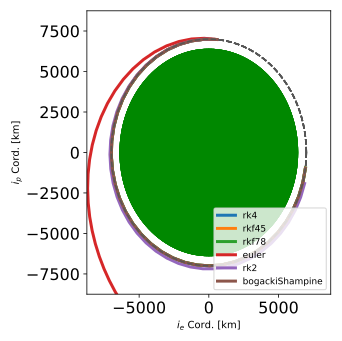
\includegraphics[]{../../../../SimScenarios/_Documentation/AutoTex/scenarioIntegrators}
	}
	\caption{Illustration of the BSK integrated trajectories.}
	\label{fig:intResults}
\end{figure}

\begin{table}[h]
	\caption{Integration test results.}
	\label{tbl:intResults}
	\centering \fontsize{10}{10}\selectfont
	\begin{tabular}{c | c | p{4in} } % Column formatting, 
		\hline\hline
		\textbf{Test} 			& \textbf{Pass/Fail} 	 & \textbf{BSK Error Notes} 									        
		\\ \hline
		``rk4"		  	& 
		\input{../../../../SimScenarios/_Documentation/AutoTex/scenarioIntegratorsTestMsg-rk4}      	  &
		\input{../../../../SimScenarios/_Documentation/AutoTex/scenarioIntegratorsMsg-rk4}
	         \\ \hline
		``euler''	   	           	&
		\input{../../../../SimScenarios/_Documentation/AutoTex/scenarioIntegratorsTestMsg-euler}           		&      
		\input{../../../../SimScenarios/_Documentation/AutoTex/scenarioIntegratorsMsg-euler}  
		\\ \hline
		``rk2''      	&
		\input{../../../../SimScenarios/_Documentation/AutoTex/scenarioIntegratorsTestMsg-rk2}
		   &  
		\input{../../../../SimScenarios/_Documentation/AutoTex/scenarioIntegratorsMsg-rk2}
\\ 
		\hline\hline
	\end{tabular}
\end{table} %This displays the test results. This includes both pass/fail statements as well as visual outputs via AutoTeX

\section{User Guide}
When using this model, the user should follow the setup procedure corresponding to his or her desired conversion described below. The procedures outline the required inputs and for each conversion and some recommended parameter values.
\subsection{Element to Cartesian}
	\begin{itemize}
		\item \textit{Elements2Cart} = \textit{True}
		\item \textit{useEphemFormat}
		\begin{itemize}
			\item \textit{True} for planet state data
			\item \textit{False} for spacecraft state data
		\end{itemize}
		\item \textit{inputsGood} = True
		\item $\mu$ is recommended to be $3.86\text{e+}14$ $\frac{\text{m}^3}{\text{s}^2}$.
		\item Keplerian orbital elements should abide by the cases layed out in the Model Functions section.
	\end{itemize}
\subsection{Cartesian to Element}
	\begin{itemize}
		\item \textit{Elements2Cart} = \textit{False}
		\item \textit{useEphemFormat}
		\begin{itemize}
			\item \textit{True} for planet state data
			\item \textit{False} for spacecraft state data
		\end{itemize}
		\item \textit{inputsGood} = \textit{True}
		\item $\mu$ is recommended to be $3.86\text{e+}14$ $\frac{\text{m}^3}{\text{s}^2}$.
		\item Recommended Cartesian vectors can be obtained from Figures \ref{fig:2} through \ref{fig:13}, which correspond to the allowed orbit types.
	\end{itemize}

\subsection{Variable Definition and Code Description}
The variables in Table \ref{tabular:vars} are available for user input. Variables used by the module but not available to the user are not mentioned here. Variables with default settings do not necessarily need to be changed by the user, but may be.
\begin{table}[H]
	\caption{Definition and Explanation of Variables Used.}
	\label{tab:errortol}
	\centering \fontsize{10}{10}\selectfont
	\begin{tabular}{  m{3cm}| m{3cm} | m{3cm} | m{6cm} } % Column formatting, 
		\hline
		\textbf{Variable}   							& \textbf{LaTeX Equivalent} 	&		\textbf{Variable Type} & \textbf{Notes}			  \\ \hline
		r$_N$	&$\bm{r}$ & double & [km]Default setting: 0.0. Position vector either used as an input to or obtained as an output from the conversions.\\ \hline
		v$_N$	& $\bm{\dot{r}}$ & double & [km/s]Default setting: 0.0. Velocity vector either used as an input to or obtained as an output from the conversions.\\ 
		\hline
		$\mu$	& $\mu$ & double & [m3/s2] Required Input. This is the gravitational parameter of the body. Replaces the product of Earth's gravitational force and mass for this test..\\
		\hline
		a & $a$ & double & [km] Required Input. The semimajor axis of the body's orbit.\\ 
		\hline
		e & $e$ & double & Required Input. The eccentricity of the body's orbit.\\ 
		\hline
		i & $i$ & double & [rad] Required Input. The inclination of the body's orbit\\ 
		\hline
		Omega & $\Omega$ & double & [rad] Required Input. The ascending node of the body's orbit. \\ 
		\hline
		omega & $\omega$ & double & [rad] Required Input. The argument of periapses of the body's orbit. \\ 
		\hline
		f & $f$ & double & [rad] Required Input. The true anomaly of the body's orbit \\
		\hline
		Elements2Cart & N/A & bool & Default Setting: False. Identifies the desired conversion. \\ 
		\hline
		useEphemFormat & N/A & bool & Default Setting: False. Identifies whether the body is a spacecraft or a planet.\\
		\hline
		inputsGood & N/A & bool & Default Setting: False. Indicates whether the code reads valid state data for conversion.\\
		\hline
	\end{tabular}
	\label{tabular:vars}
\end{table}
\begin{thebibliography}{1}
	\bibitem{bib:1}
	Vallado, D. A., and McClain, W. D., \textit{Fundamentals of Astrodynamics and Applications, 4th ed}. Hawthorne, CA: Published by Microcosm Press, 2013.
	\bibitem{bib:2}
	Schaub, H., and Junkins, J. L., \textit{Analytical Mechanics of Space Systems, 3rd ed.}. Reston, VA: American Institute of Aeronautics and Astronautics.
\end{thebibliography} %This section is to provide advice to users on necessary/useful inputs and best practices.

\bibliography{bibliography.bib} %This includes references used and mentioned.

\end{document}
